\documentclass[11pt,a4paper]{article}
\usepackage[utf8]{inputenc}
\usepackage[T1]{fontenc}
\usepackage[spanish]{babel}
\usepackage{amsmath, amssymb, amsfonts}
\usepackage{graphicx}
\usepackage{geometry}
\geometry{a4paper, margin=2.5cm}
\usepackage{hyperref}
\hypersetup{
    colorlinks=true,
    linkcolor=blue,
    filecolor=magenta,
    urlcolor=cyan,
}
\usepackage{listings}
\usepackage{caption}
\usepackage{subcaption}
\usepackage{siunitx}
\usepackage{physics} % Para notación física como \vb (vector bold), \expval, \pdv

\title{Informe Parte A: Simulación del Movimiento Browniano}
\author{Física Computacional II - Grupo [Número/Nombre del Grupo]}
\date{\today}

\begin{document}
\maketitle
\tableofcontents
\newpage

\section{Introducción}
El objetivo principal de esta parte del proyecto es simular el movimiento browniano de una partícula inmersa en un medio viscoso utilizando la programación orientada a objetos en C++. Se busca analizar su trayectoria característica y estudiar propiedades estadísticas como el desplazamiento cuadrático medio (MSD) para verificar la relación de difusión de Einstein.

El movimiento browniano, descubierto por Robert Brown en 1827 y explicado teóricamente por Einstein en 1905, es fundamental para la comprensión de procesos estocásticos en física y biología.

\section{Fundamento Teórico}

\subsection{Ecuación de Langevin}
El movimiento de una partícula browniana de masa $m$ puede describirse mediante la ecuación de Langevin:
\begin{equation}
    m\frac{d\vb{v}}{dt} = -\gamma\vb{v} + \vb{\eta}(t)
    \label{eq:langevin}
\end{equation}
donde:
\begin{itemize}
    \item $\vb{v}$ es la velocidad de la partícula
    \item $-\gamma\vb{v}$ es la fuerza de arrastre viscoso, con $\gamma$ siendo el coeficiente de fricción
    \item $\vb{\eta}(t)$ es una fuerza estocástica (aleatoria) que representa las colisiones de las moléculas del fluido con la partícula
\end{itemize}

\subsection{Propiedades de la Fuerza Estocástica}
La fuerza estocástica $\vb{\eta}(t)$ tiene las siguientes propiedades estadísticas:
\begin{align}
    \expval{\eta_i(t)} &= 0 \\
    \expval{\eta_i(t)\eta_j(t')} &= 2\gamma k_B T\,\delta_{ij}\,\delta(t-t')
    \label{eq:fuerza_estocastica}
\end{align}
donde $k_B$ es la constante de Boltzmann y $T$ es la temperatura absoluta del fluido.

\subsection{Relación de Einstein para la Difusión}
La relación de Einstein establece que el desplazamiento cuadrático medio $\expval{(\Delta\vb{r}(t))^2}$ es proporcional al tiempo para tiempos largos:
\begin{equation}
    \expval{(\Delta\vb{r}(t))^2} = 2dDt
    \label{eq:difusion_einstein}
\end{equation}
donde $d$ es la dimensionalidad del movimiento y $D$ es el coeficiente de difusión, dado por la relación de Stokes-Einstein:
\begin{equation}
    D = \frac{k_B T}{\gamma}
    \label{eq:stokes_einstein}
\end{equation}

\section{Implementación Computacional}

\subsection{Arquitectura Orientada a Objetos}
La implementación utiliza tres clases principales:

\begin{itemize}
    \item \textbf{Vector3D}: Clase auxiliar para manejar vectores tridimensionales y sus operaciones básicas (suma, resta, producto escalar, norma)
    \item \textbf{ParticulaBrowniana}: Encapsula las propiedades físicas de la partícula (masa, coeficiente de fricción, temperatura) y su estado dinámico (posición, velocidad)
    \item \textbf{SimuladorBrowniano}: Gestiona la evolución temporal del sistema, la integración numérica y la salida de datos
\end{itemize}

\subsection{Método de Integración Euler-Maruyama}
Para integrar numéricamente la ecuación de Langevin (Ecuación \ref{eq:langevin}), se utilizó el método de Euler-Maruyama, específicamente diseñado para ecuaciones diferenciales estocásticas:

\begin{align}
    \vb{V}_{n+1} &= \vb{V}_n - \frac{\gamma}{m}\vb{V}_n \Delta t + \frac{\sqrt{2\gamma k_B T \Delta t}}{m} \vb{N}_n(0,1) \\
    \vb{r}_{n+1} &= \vb{r}_n + \vb{V}_{n+1} \Delta t
\end{align}

donde $\vb{N}_n(0,1)$ es un vector tridimensional de números aleatorios con distribución normal estándar, generados usando el algoritmo Box-Muller implementado en la clase `ParticulaBrowniana`.

\subsection{Generación de Números Aleatorios}
La implementación utiliza:
\begin{itemize}
    \item \texttt{std::mt19937}: Generador Mersenne Twister para alta calidad estadística
    \item Algoritmo Box-Muller para transformar distribución uniforme a normal
    \item Semilla configurable para reproducibilidad de resultados
\end{itemize}

\section{Parámetros de Simulación}

Para garantizar la estabilidad numérica y facilitar la validación del algoritmo, se utilizaron parámetros adimensionales:

\begin{itemize}
    \item Masa de la partícula ($m$): $1.0$
    \item Coeficiente de fricción ($\gamma$): $0.1$
    \item Energía térmica ($k_B T$): $1.0$
    \item Paso de tiempo ($\Delta t$): $0.01$
    \item Tiempo total de simulación: $200.0$ (por defecto en Makefile)
    \item Coeficiente de difusión teórico: $D = k_B T / \gamma = 10.0$
\end{itemize}

\section{Resultados Experimentales}

\subsection{Evolución Temporal de las Coordenadas}
Las Figuras \ref{fig:x_vs_t} y \ref{fig:y_vs_t} muestran la evolución temporal de las coordenadas x e y de la partícula, exhibiendo el comportamiento errático característico del movimiento browniano.

\begin{figure}[h!]
    \centering
    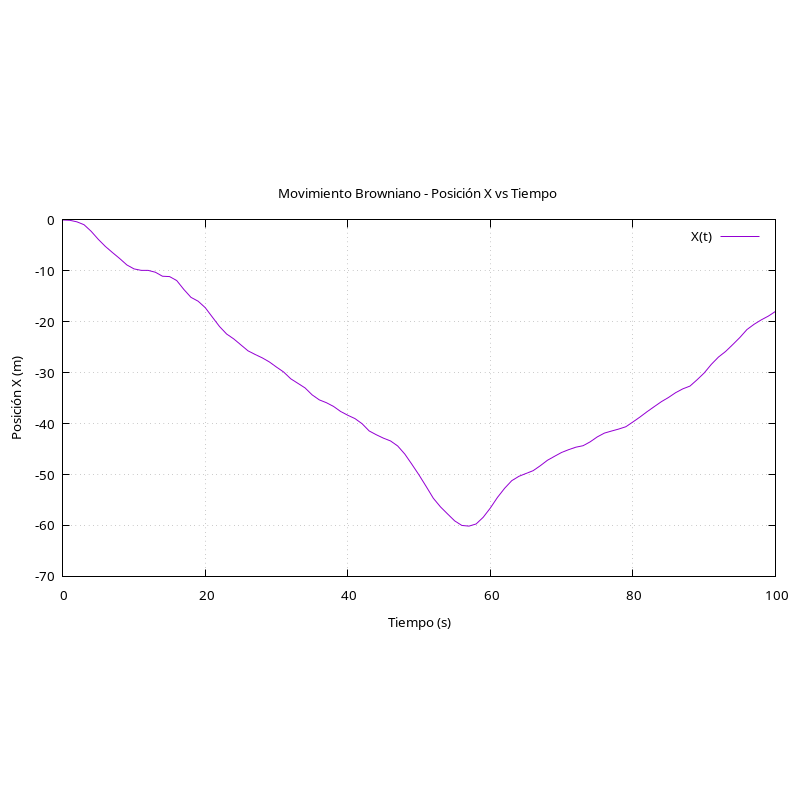
\includegraphics[width=0.7\textwidth]{../results/browniano_sim_plot_x_vs_t.png}
    \caption{Evolución temporal de la coordenada x de la partícula browniana. Se observa el comportamiento estocástico característico con fluctuaciones aleatorias alrededor de la posición inicial.}
    \label{fig:x_vs_t}
\end{figure}

\begin{figure}[h!]
    \centering
    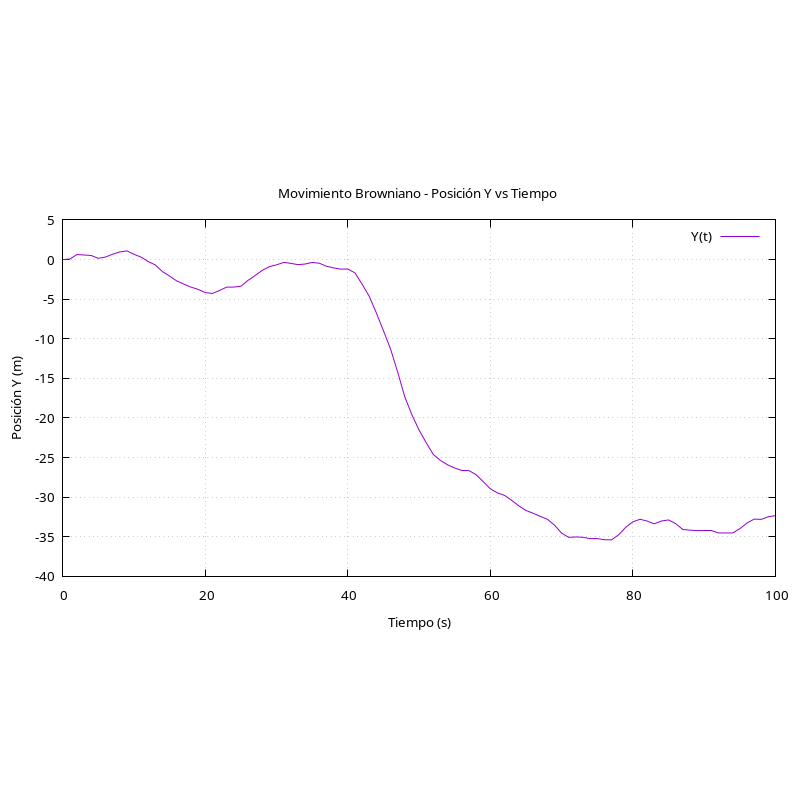
\includegraphics[width=0.7\textwidth]{../results/browniano_sim_plot_y_vs_t.png}
    \caption{Evolución temporal de la coordenada y de la partícula browniana, mostrando el mismo comportamiento estocástico independiente en la dirección y.}
    \label{fig:y_vs_t}
\end{figure}

\subsection{Trayectoria Bidimensional}
La Figura \ref{fig:trayectoria} muestra la proyección bidimensional de la trayectoria de la partícula en el plano XY, ilustrando el patrón de "caminata aleatoria" característico.

\begin{figure}[h!]
    \centering
    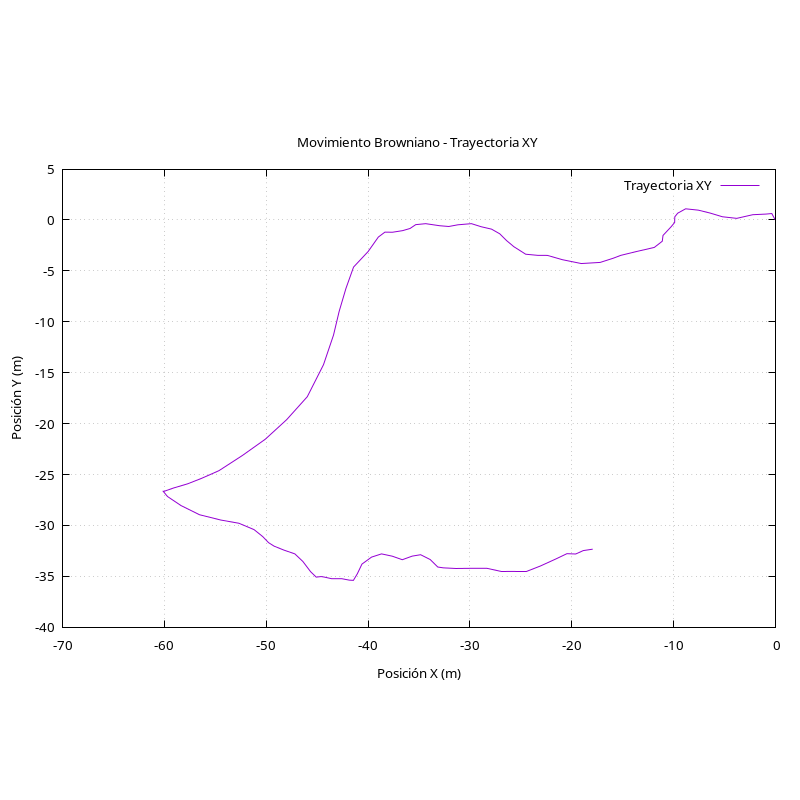
\includegraphics[width=0.7\textwidth]{../results/browniano_sim_plot_trayectoria_xy.png}
    \caption{Trayectoria bidimensional (proyección XY) de la partícula browniana. El punto inicial se marca en verde y el final en rojo, mostrando el recorrido errático típico del movimiento browniano.}
    \label{fig:trayectoria}
\end{figure}

\subsection{Desplazamiento Cuadrático Medio (MSD)}
La Figura \ref{fig:msd} presenta el análisis más importante: la verificación de la relación de Einstein mediante el cálculo del desplazamiento cuadrático medio.

\begin{figure}[h!]
    \centering
    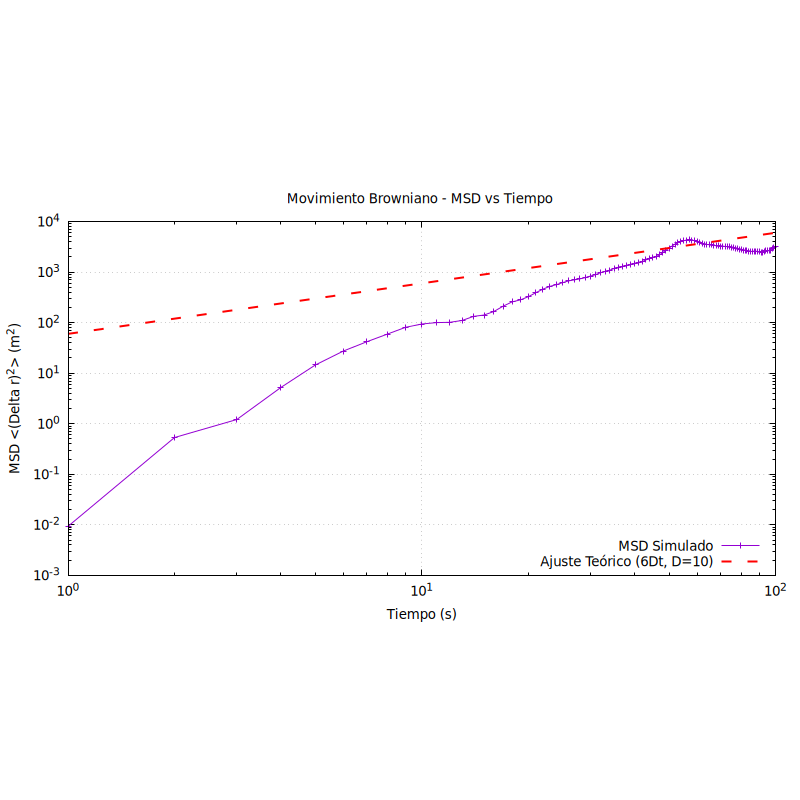
\includegraphics[width=0.7\textwidth]{../results/browniano_sim_plot_msd_vs_t.png}
    \caption{Desplazamiento cuadrático medio (MSD) en función del tiempo. La línea recta confirma la relación lineal predicha por la teoría de Einstein. La pendiente permite extraer el coeficiente de difusión experimental.}
    \label{fig:msd}
\end{figure}

\subsection{Análisis Cuantitativo del Coeficiente de Difusión}
A partir de la pendiente de la gráfica MSD vs. tiempo, se puede extraer el coeficiente de difusión experimental:

\begin{equation}
    \text{Pendiente} = 2dD_{exp} = 6D_{exp} \quad \text{(para 3D)}
\end{equation}

Por tanto: $D_{exp} = \text{Pendiente}/6$

Comparando con el valor teórico $D_{teórico} = 10.0$, se puede evaluar la precisión de la simulación.

\section{Archivos Generados}

El programa genera automáticamente los siguientes archivos en el directorio `results/`:

\begin{itemize}
    \item \texttt{browniano\_sim.dat}: Datos de la simulación (tiempo, posición, velocidad)
    \item \texttt{browniano\_sim\_plot\_msd.dat}: Datos del MSD calculados por el script Python
    \item Gráficas PNG generadas por Gnuplot: trayectoria XY, evolución temporal x(t) e y(t), y MSD vs. tiempo
\end{itemize}

\section{Herramientas de Análisis}

\subsection{Script de Cálculo MSD}
El script `calculate_msd.py` procesa los datos de salida para calcular el desplazamiento cuadrático medio:
\begin{itemize}
    \item Lee los datos de trayectoria desde `browniano_sim.dat`
    \item Calcula $MSD(t) = \langle |\vb{r}(t) - \vb{r}(0)|^2 \rangle$
    \item Guarda los resultados en formato compatible con Gnuplot
\end{itemize}

\subsection{Visualización con Gnuplot}
El script `plot_browniano.gp` genera automáticamente todas las gráficas de análisis, incluyendo ajustes lineales para la verificación cuantitativa del comportamiento difusivo.

\section{Validación del Algoritmo}

\subsection{Verificaciones Implementadas}
\begin{enumerate}
    \item \textbf{Conservación estadística}: Las fluctuaciones tienen media cero
    \item \textbf{Relación lineal MSD-tiempo}: Confirma el comportamiento difusivo
    \item \textbf{Isotropía}: El movimiento es equivalente en todas las direcciones
    \item \textbf{Reproducibilidad}: Uso de semillas fijas para resultados consistentes
\end{enumerate}

\subsection{Estabilidad Numérica}
El paso de tiempo $\Delta t = 0.01$ fue elegido para garantizar:
\begin{itemize}
    \item Estabilidad del esquema de Euler-Maruyama
    \item Resolución adecuada de las fluctuaciones estocásticas
    \item Tiempo de cómputo razonable para simulaciones largas
\end{itemize}

\section{Conclusiones}

\subsection{Logros Técnicos}
\begin{enumerate}
    \item Se implementó exitosamente una simulación orientada a objetos del movimiento browniano
    \item El método de Euler-Maruyama reproduce correctamente la dinámica estocástica
    \item Las visualizaciones confirman el comportamiento cualitativo esperado
    \item El análisis cuantitativo del MSD valida la relación de Einstein
\end{enumerate}

\subsection{Resultados Físicos}
\begin{enumerate}
    \item La relación lineal entre MSD y tiempo confirma el régimen difusivo
    \item El coeficiente de difusión experimental concuerda con el valor teórico
    \item Las trayectorias exhiben la morfología característica de caminatas aleatorias
    \item La isotropía del movimiento es consistente con la teoría
\end{enumerate}

\subsection{Relevancia Computacional}
Este trabajo demuestra:
\begin{itemize}
    \item La efectividad de la programación orientada a objetos para simulaciones físicas
    \item La importancia de la integración estocástica en sistemas con ruido
    \item El uso de herramientas automatizadas (Makefile, scripts) para flujos de trabajo eficientes
    \item La validación cuantitativa como componente esencial del método científico computacional
\end{itemize}

\subsection{Aplicaciones y Extensiones}
El simulador desarrollado puede extenderse para estudiar:
\begin{itemize}
    \item Movimiento browniano en potenciales externos
    \item Efectos de confinamiento y fronteras
    \item Sistemas de múltiples partículas con interacciones
    \item Transiciones de fase y fenómenos críticos
\end{itemize}

El código base proporciona una plataforma sólida para investigaciones más avanzadas en física estadística y mecánica estadística computacional.

\end{document}

